\section{基本群}
\label{section:ch09-sec52}

空间 $X$ 中道路的道路同伦类的集合对于运算 $*$ 而言并不是一个群, 因为两个道路同伦类的乘积并不总有定义. 但是, 如果我们取定 $X$ 中的点 $x_0$ 作为"基点", 并且只考虑那些起点和终点都是 $x_0$ 的道路, 那么这种道路的道路同伦类的集合对于运算 $*$ 而言便构成了一个群, 这个群称为 $X$ 的基本群.

在这一节中, 我们将要研究基本群的一些性质. 特别地, 我们要证明基本群是空间 $X$ 的拓扑不变量. 对于研究同胚问题, 这一结果是十分重要的.

我们先来回顾群论中的某些术语. 设 $G$ 和 $G'$ 都是群, 其中的运算用乘法表示. \textbf{同态}(homomorphism) $f\colon G\to G'$ 是一个映射, 使得对于所有 $x$, $y\in G$, $f(x\cdot y)=f(x)\cdot f(y)$. 对于同态而言, 等式 $f(e)=e'$ 和 $f(x^{-1})=f(x)^{-1}$ 一定会成立, 其中 $e$ 和 $e'$ 分别是 $G$ 和 $G'$ 中的单位元, 并且指数 $-1$ 表示逆元. $f$ 的\textbf{核}(kernel) 是 $f^{-1}(e')$, 它是 $G$ 的一个子群. 同样, $f$ 的像是 $G'$ 的一个子群. 同态 $f$ 叫做\textbf{单同态}(monomorphism), 如果它是一个单射 (这等价于 $f$ 的核由 $e$ 单独构成). 同态 $f$ 叫做\textbf{满同态}(epimorphism), 如果它是一个满射. 同态 $f$ 叫做\textbf{同构}(isomorphism), 如果它是一个一一映射.

设 $G$ 是一个群, $H$ 是 $G$ 的一个子群. 用 $xH$ 表示所有乘积 $x\cdot h$ 构成的集合, $h\in H$, 这个集合称为 $H$ 在 $G$ 中的一个\textbf{左陪集}(left coset). 所有左陪集构成的族形成 $G$ 的一个分拆. 类似地, $H$ 在 $G$ 中的所有右陪集 $Hx$ 构成的族也形成 $G$ 的一个分拆. 如果对于每一个 $x\in G$ 和每一个 $h\in H$, 有 $x\cdot h\cdot x^{-1}\in H$, 则称 $H$ 是 $G$ 的一个\textbf{正规子群}(normal subgroup). 在这种情形下我们有 $xH=Hx$, 因此上述的两个分拆是一样的. 这时将这个分拆表示为 $G/H$. 如果定义
\[
(xH)\cdot(yH)=(x\cdot y)H,
\]
我们便得到了 $G/H$ 中的一个定义确切的运算, 并且使得它成为一个群. 这个群称为群 $G$ 相对于子群 $H$ 而言的\textbf{商群}(quotient). 映射 $f\colon G\to G/H$ 将 $x$ 映为 $xH$, 是以 $H$ 为核的同态. 反之, 如果 $f\colon G\to G'$ 是一个满同态, 则这个同态的核 $N$ 便是 $G$ 的一个正规子群, 并且 $f$ 诱导出一个同构 $G/N\to G'$, 对于每一个 $x\in G$ 这个同构将 $xN$ 映为 $f(x)$.

如果子群 $H$ 不是正规的, 我们用记号 $G/H$ 表示 $H$ 在 $G$ 中的右陪集构成的族.

\begin{definition}[基本群]
\label{definition:ch09-sec52-pi1}
设 $X$ 为一个空间, $x_0$ 为 $X$ 的一个点. $X$ 中起点和终点都是 $x_0$ 的道路称为以 $x_0$ 为基点的\textbf{回路}(loop). 所有以 $x_0$ 为基点的回路的道路同伦类组成的集合对于运算"$*$"而言构成一个群, 称为空间 $X$ 关于\textbf{基点}(base point) $x_0$ 的\textbf{基本群}(fundamental group), 记作 $\pi_1(X,x_0)$.
\end{definition}

从定理 \cref{theorem:ch09-sec51-51-2} 可见, 运算"$*$"限制在上述定义中谈到的集合上, 满足群的以下公理: 对于任意给定的两条以 $x_0$ 为基点的回路 $f$ 和 $g$, 乘积 $f*g$ 总是有定义的, 并且它也是以 $x_0$ 为基点的一条回路. 结合律、单位元 $[e_{x_0}]$ 的存在性、$[f]$ 的逆元 $[\bar{f}]$ 的存在性都是明显的.

有时, $X$ 的基本群也称为 $X$ 的\textbf{第一个同伦群}(first homotopy group). 这意味着还会有第二个同伦群. 事实上, 对于每一个 $n\in\mathbb{Z}_{+}$, 都会有群 $\pi_n(X,x_0)$. 但是我们在本书中不去研究它们, 它们称为同伦论的一门学问中的研究对象的一部分.

\begin{example}
\label{example:ch09-sec52-1}
设 $\mathbb{R}^{n}$ 为 $n$-维欧氏空间. 则 $\pi_1(\mathbb{R}^{n},x_0)$ 是平凡群 (即由单位元一个元素构成的群), 因为如果 $f$ 是 $\mathbb{R}^{n}$ 中以 $x_0$ 为基点的一条回路, 那么直线同伦便是 $f$ 与 $x_0$ 处的常值道路之间的一个道路同伦. 更一般地, 如果 $X$ 是 $\mathbb{R}^{n}$ 中的一个凸集, 那么 $\pi_1(X,x_0)$ 便是平凡群. 特别地, $\mathbb{R}^{n}$ 中的\textbf{单位球}(unit ball)
\[
B^{n}=\{\,\boldsymbol{x}\mid x_{1}^{2}+\cdots+x_{n}^{2}\leqslant 1\,\}
\]
的基本群是平凡群.
\end{example}

人们马上要问: 基本群在多大程度上依赖于基点? 我们现在来给出这个问题的回答.

\begin{definition}[道路诱导的同构]
\label{definition:ch09-sec52-alpha-hat}
设 $\alpha$ 是 $X$ 中从 $x_0$ 到 $x_1$ 的一条道路. 定义映射
\[
\hat{\alpha}\colon\pi_{1}(X,x_{0})\longrightarrow\pi_{1}(X,x_{1}),
\]
使得
\[
\hat{\alpha}([f])=[\bar{\alpha}]*[f]*[\alpha].
\]
\end{definition}

因为运算"$*$"的定义是确切的, 映射 $\hat{\alpha}$ 的定义也是确切的, 它叫做"$\alpha$-帽". 如果 $f$ 是以 $x_0$ 为基点的一条回路, 那么 $\bar{\alpha}*(f*\alpha)$ 便是以 $x_1$ 为基点的一条回路. 因此 $\hat{\alpha}$ 将 $\pi_1(X,x_0)$ 映射到 $\pi_1(X,x_1)$ 中, 这正是我们所需要的. 注意, $\hat{\alpha}$ 仅依赖于 $\alpha$ 的道路同伦类. 参见图 \cref{figure:ch09-fig-52-1}.

\par
\begin{figure}[htbp]
\centering
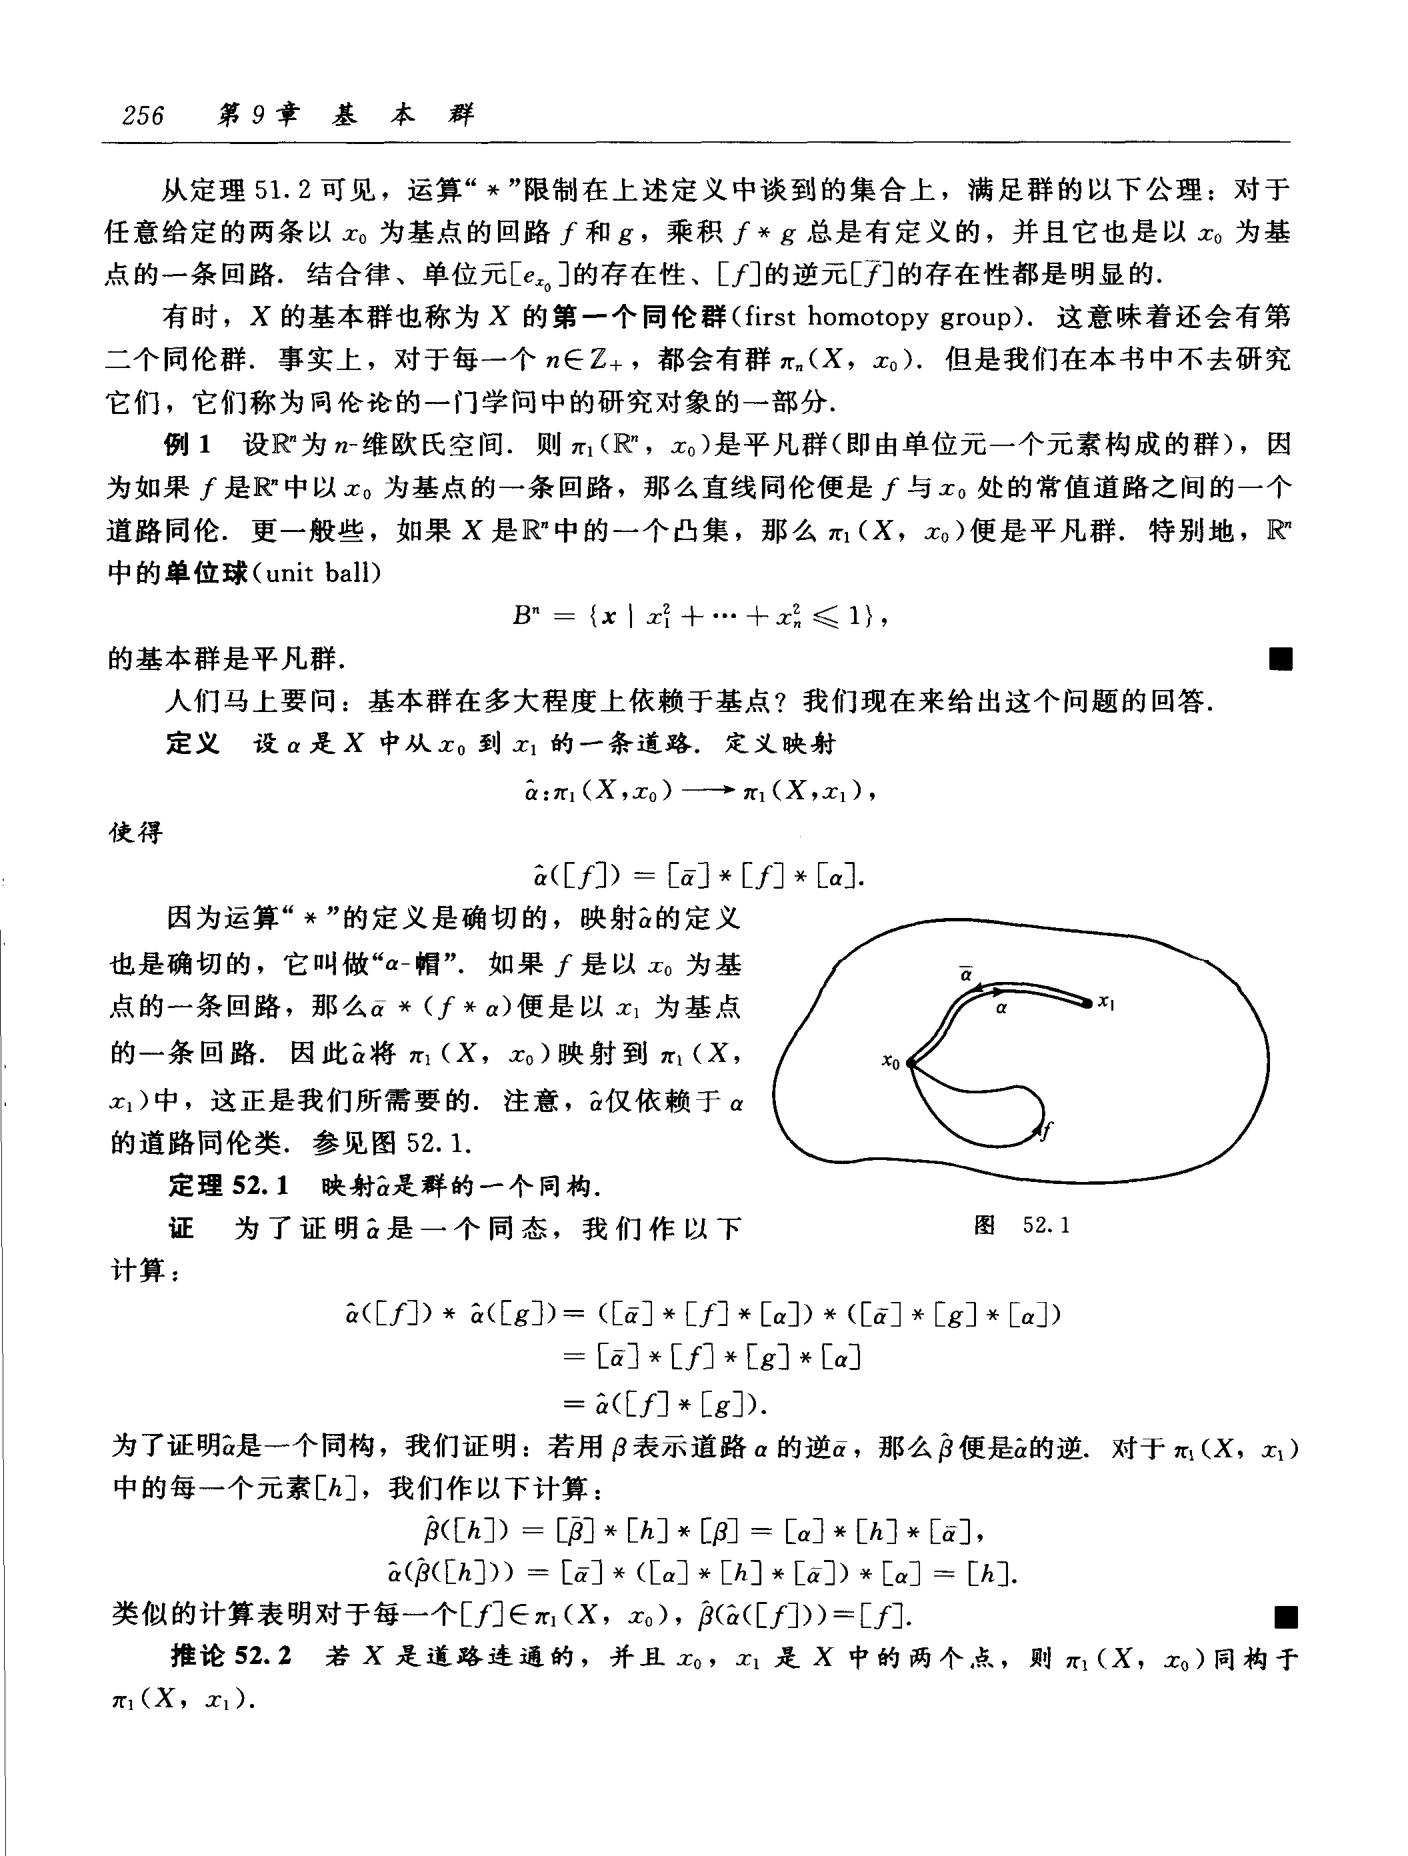
\includegraphics[width=0.5\textwidth]{image/fig-52-1.png}
\caption{$\hat{\alpha}$ 的定义.}
\label{figure:ch09-fig-52-1}
\end{figure}

\begin{theorem}
\label{theorem:ch09-sec52-52-1}
映射 $\hat{\alpha}$ 是群的一个同构.
\end{theorem}

\begin{proof}
为了证明 $\hat{\alpha}$ 是一个同态, 我们作以下计算:
\[
\begin{aligned}
\hat{\alpha}([f])*\hat{\alpha}([g])
&=([\bar{\alpha}]*[f]*[\alpha])*([\bar{\alpha}]*[g]*[\alpha])\\
&=[\bar{\alpha}]*[f]*[g]*[\alpha]\\
&=\hat{\alpha}([f]*[g]).
\end{aligned}
\]
为了证明 $\hat{\alpha}$ 是一个同构, 我们证明: 若用 $\beta$ 表示道路 $\alpha$ 的逆 $\bar{\alpha}$, 那么 $\hat{\beta}$ 便是 $\hat{\alpha}$ 的逆. 对于 $\pi_1(X,x_1)$ 中的每一个元素 $[h]$, 我们作以下计算:
\[
\hat{\beta}([h])=[\bar{\beta}]*[h]*[\beta]=[\alpha]*[h]*[\bar{\alpha}],
\]
\[
\hat{\alpha}(\hat{\beta}([h]))=[\bar{\alpha}]*([\alpha]*[h]*[\bar{\alpha}])*[\alpha]=[h].
\]
类似的计算表明对于每一个 $[f]\in\pi_1(X,x_0)$, $\hat{\beta}(\hat{\alpha}([f]))=[f]$.
\end{proof}

\begin{corollary}
\label{corollary:ch09-sec52-52-2}
若 $X$ 是道路连通的, 并且 $x_0$, $x_1$ 是 $X$ 中的两个点, 则 $\pi_1(X,x_0)$ 同构于 $\pi_1(X,x_1)$.
\end{corollary}

设 $X$ 是一个拓扑空间, $C$ 为 $X$ 中包含 $x_0$ 的道路连通分支, 易见 $\pi_1(C,x_0)=\pi_1(X,x_0)$, 因为 $X$ 中所有以 $x_0$ 为基点的回路和同伦都包含在子空间 $C$ 中. 于是 $\pi_1(X,x_0)$ 只依赖于 $X$ 中包含 $x_0$ 的道路连通分支, 并且 $\pi_1(X,x_0)$ 也不反映 $X$ 的其余部分的任何情况. 因此, 当我们研究基本群时, 通常只考虑道路连通的空间.

如果 $X$ 道路连通, 那么所有的基本群 $\pi_1(X,x)$ 都是同构的. 这自然使人试图将这些群彼此"等同"起来, 以便能够不涉及基点而简单地谈论空间 $X$ 的基本群. 做这件事的困难在于没有等同 $\pi_1(X,x_0)$ 与 $\pi_1(X,x_1)$ 的自然的方式, 从 $x_0$ 到 $x_1$ 的不同道路可以给出这两个群之间不同的同构. 因此, 忽略基点会导致错误.

已经知道, $\pi_1(X,x_0)$ 与 $\pi_1(X,x_1)$ 的同构与道路的选取无关当且仅当基本群是一个交换群 (见习题 3). 这是对空间 $X$ 的一种苛刻的要求.

\begin{definition}[单连通]
\label{definition:ch09-sec52-simply-connected}
如果 $X$ 是道路连通空间, 并且对于某一个 $x_0\in X$, $\pi_1(X,x_0)$ 是平凡群 (只有一个元素), 从而对于每一个 $x_0\in X$, $\pi_1(X,x_0)$ 是平凡群, 则称 $X$ 是\textbf{单连通的}(simply connected). $\pi_1(X,x_0)$ 是平凡群这一事实常表示为 $\pi_1(X,x_0)=0$.
\end{definition}

\begin{lemma}
\label{lemma:ch09-sec52-52-3}
在单连通空间 $X$ 中, 任何两条有公共起点和终点的道路都是道路同伦的.
\end{lemma}

\begin{proof}
设 $\alpha$ 和 $\beta$ 是从 $x_0$ 到 $x_1$ 的两条道路. 则 $\alpha*\bar{\beta}$ 有定义, 并且是 $X$ 中以 $x_0$ 为基点的一条回路. 由于 $X$ 是单连通的, 所以这条回路道路同伦于 $x_0$ 处的常值回路. 因此
\[
[\alpha*\bar{\beta}]*[\beta]=[e_{x_{0}}]*[\beta],
\]
由此可见 $[\alpha]=[\beta]$.
\end{proof}

基本群是空间 $X$ 的拓扑不变量, 这在直观上看起来十分清楚. 为了严格证明这一点, 一个方便的方式便是引入"连续映射诱导同态"这一概念.

设 $h\colon X\to Y$ 为连续映射, 并且 $h$ 将 $X$ 中的点 $x_0$ 变为 $Y$ 中的点 $y_0$. 我们常用记号
\[
h\colon(X,x_{0})\longrightarrow(Y,y_{0})
\]
来表示这种情形. 如果 $f$ 是 $X$ 中以 $x_0$ 为基点的一条回路, 那么复合映射 $h\circ f\colon I\to Y$ 便是 $Y$ 中以 $y_0$ 为基点的一条回路. 这样一来, 对应 $f\mapsto h\circ f$ 便会引出将 $\pi_1(X,x_0)$ 映到 $\pi_1(Y,y_0)$ 的一个映射. 下面正式给出定义.

\begin{definition}[诱导同态]
\label{definition:ch09-sec52-induced}
设 $h\colon(X,x_0)\to(Y,y_0)$ 是一个连续映射. 定义
\[
h_{*}\colon\pi_{1}(X,x_{0})\longrightarrow\pi_{1}(Y,y_{0})
\]
使得
\[
h_{*}([f])=[h\circ f].
\]
映射 $h_*$ 称为 $h$ 相对于基点 $x_0$ 而言的\textbf{诱导同态}(induced homomorphism).
\end{definition}

映射 $h_*$ 的定义是确切的. 因为如果 $F$ 是道路 $f$ 与 $f'$ 之间的一个道路同伦, 那么 $h\circ F$ 便是道路 $h\circ f$ 与 $h\circ f'$ 之间的一个道路同伦. 也容易证明 $h_*$ 是一个同态, 因为
\[
(h\circ f)*(h\circ g)=h\circ(f*g).
\]
诱导同态 $h_*$ 不仅依赖于映射 $h\colon X\to Y$, 也依赖于基点 $x_0$ 的选取. (当 $x_0$ 取定时, $y_0$ 由 $f$ 确定.) 因此, 当我们考虑 $X$ 中几个不同的基点时, 记号上就会出现一些麻烦. 如果 $x_0$, $x_1$ 是 $X$ 中不相同的两点, 我们总不能用同一个符号 $h_*$ 去表示两个不同的同态, 其中第一个的定义域是 $\pi_1(X,x_0)$, 而第二个的定义域是 $\pi_1(X,x_1)$. 即使当 $X$ 道路连通, 因而所有这些群都同构的时候, 也会有这样的问题, 因为毕竟这些群并不相同. 因此, 我们将采用记号
\[
(h_{x_{0}})_{*}\colon\pi_{1}(X,x_{0})\longrightarrow\pi_{1}(X,y_{0})
\]
表示前述的第一个同态, 而用 $(h_{x_1})_*$ 表示第二个同态. 如果在讨论某问题时只考虑一个基点, 我们常常不提基点而简单地用 $h_*$ 表示诱导同态.

诱导同态有两个十分重要的性质, 称为诱导同态的"函子性质". 这两个性质在下列定理中给出.

\begin{theorem}
\label{theorem:ch09-sec52-52-4}
若 $h\colon(X,x_0)\to(Y,y_0)$ 和 $k\colon(Y,y_0)\to(Z,z_0)$ 都是连续的, 则 $(k\circ h)_*=k_*\circ h_*$. 如果 $i\colon(X,x_0)\to(X,x_0)$ 是恒等映射, 则 $i_*$ 是恒等同态.
\end{theorem}

\begin{proof}
证明是简单的. 根据定义
\[
(k\circ h)_{*}([f])=[(k\circ h)\circ f],
\]
\[
(k_{*}\circ h_{*})([f])=k_{*}(h_{*}([f]))=k_{*}([h\circ f])=[k\circ(h\circ f)],
\]
类似地, $i_*([f])=[i\circ f]=[f]$.
\end{proof}

\begin{corollary}
\label{corollary:ch09-sec52-52-5}
若 $h\colon(X,x_0)\to(Y,y_0)$ 是 $X$ 与 $Y$ 之间的一个同胚, 则 $h_*$ 是 $\pi_1(X,x_0)$ 与 $\pi_1(Y,y_0)$ 之间的一个同构.
\end{corollary}

\begin{proof}
设 $k\colon(Y,y_0)\to(X,x_0)$ 为 $h$ 的逆, 则 $k_*\circ h_*=(k\circ h)_*=i_*$, 其中 $i$ 是 $(X,x_0)$ 的恒等映射. 而 $h_*\circ k_*=(h\circ k)_*=j_*$, 其中 $j$ 是 $(Y,y_0)$ 的恒等映射. 由于 $i_*$ 和 $j_*$ 分别是 $\pi_1(X,x_0)$ 和 $\pi_1(Y,y_0)$ 的恒等同态, 所以 $k_*$ 是 $h_*$ 的逆.
\end{proof}

\subsection*{习题}

\begin{exercise}
$\mathbb{R}^{n}$ 的一个子集 $A$ 称为\textbf{星形凸集}(star convex), 如果 $A$ 中有一个点 $a_0$, 使得连接 $a_0$ 与 $A$ 中任意另外一点的线段都包含在 $A$ 中.
\begin{enumerate}
\item 找出一个不是凸集的星形凸集.
\item 证明: 若 $A$ 是星形凸集, 则 $A$ 是单连通的.
\end{enumerate}
\end{exercise}

\begin{exercise}
设 $\alpha$ 是 $X$ 中的一条从 $x_0$ 到 $x_1$ 的道路, $\beta$ 是 $X$ 中的一条从 $x_1$ 到 $x_2$ 的道路. 证明: 如果 $\gamma=\alpha*\beta$, 则 $\hat{\gamma}=\hat{\beta}\circ\hat{\alpha}$.
\end{exercise}

\begin{exercise}
设 $x_0$ 和 $x_1$ 为道路连通空间 $X$ 中给定的两个点. 证明: $\pi_1(X,x_0)$ 是一个交换群当且仅当对于任意两条从 $x_0$ 到 $x_1$ 的道路 $\alpha$ 和 $\beta$, 有 $\hat{\alpha}=\hat{\beta}$.
\end{exercise}

\begin{exercise}
设 $A\subset X$, 又设 $r\colon X\to A$ 是连续映射, 使得对于每一个 $a\in A$, $r(a)=a$. (映射 $r$ 称为从 $X$ 到 $A$ 上的\textbf{收缩}.) 给定 $a_0\in A$, 证明
\[
r_{*}\colon\pi_{1}(X,a_{0})\longrightarrow\pi_{1}(A,a_{0})
\]
是满射.
\end{exercise}

\begin{exercise}
设 $A$ 为 $\mathbb{R}^{n}$ 的一个子空间, 又设 $h\colon(A,a_0)\to(Y,y_0)$. 证明: 若 $h$ 可扩张成一个从 $\mathbb{R}^{n}$ 到 $Y$ 中的连续映射, 则 $h_*$ 为平凡同态 (即将每一个元素都映成单位元的同态).
\end{exercise}

\begin{exercise}
证明: 若 $X$ 是道路连通的, 则在不区别所涉及的群之间的同构的前提下, 连续映射的诱导同态与基点的选取无关. 精确地说, 设 $h\colon X\to Y$ 是连续的, 有 $h(x_0)=y_0$ 和 $h(x_1)=y_1$. 设 $\alpha$ 是 $X$ 中从 $x_0$ 到 $x_1$ 的一条道路, 令 $\beta=h\circ\alpha$, 则有
\[
\hat{\beta}\circ(h_{x_{0}})_{*}=(h_{x_{1}})_{*}\circ\hat{\alpha}.
\]
\end{exercise}
